%%% CBC SEARCH %%%
% Gravitational Wave data
%    h = s + n
% Signal Model
%    Waveforms
% Noise Model
%    PSD
% Search Methods
%    Matched Filter
%    Phase Maximisation
%    Template Bank
%    Signal Consistency Tests
%    Exponential Noise Model
%    PSD Variation
%    Coincidence Tests
%        Simple One
%        PhaseTD
%    Ranking Statistic
% PyCBC
%    Offline vs Live
%    Low-Latency Detection
%    SNR Optimisation
% Gravitational-Wave Observations to date



% Chapter Introduction

\Gwadj search pipelines, such as PyCBC, play a critical role in analysing data from detectors to identify \gwadj signals, both in real time (live) and in post-processing (offline). This chapter develops the theoretical foundation for these search pipelines and explores the techniques employed in \gwadj detection. Emphasis is placed on the PyCBC pipelines---PyCBC Offline and PyCBC Live---both of which were extensively utilised and further developed as part of this thesis.

\section{\label{2:sec:gw-data}\Gwadj data}

\Gwadj observatories produce a dimensionless strain time-series, $s(t)$, which is composed of detector noise, $n(t)$, and, when present, an astrophysical \gwadj signal, $h(t)$
%
\begin{equation}
    s(t) =
    \begin{cases}
        n(t), & \text{if no signal is present}, \\
        n(t) + h(t), & \text{if a signal is present}.
    \end{cases}
\end{equation}
%
The primary objective of \gwadj search pipelines is to extract $h(t)$ from $s(t)$, detecting the astrophysical signal from within the background noise.

\section{\label{2:sec:search-methods}Searching through \gwadj data}

Detecting \gws from \cbcs requires sophisticated search methods capable of sifting through vast amounts of data collected by \gwadj detectors. This section details the search techniques used to identify and characterise \gwadj signals. There are many pipelines that search for \gws~\cite{pipelines, PyCBC:2017, GstLAL:2020, SPIIR:2020, MBTA:2021, cWB:2020, oLIB:2015, MLy:2020qax} and in this section we will focus on the PyCBC search~\cite{PyCBC:2016, PyCBC:2017, PyCBC_package:2021}

We begin with the single-detector search techniques to identify potential \gwadj events, and then detail the tests and methods used to combine single detector detections to identify coincidentally found \gwadj signals.

\subsection{\label{2:sec:matched-filter}Matched filtering}

% Use Jolien's book
Detecting \gws relies on being able to distinguish between data that contains only noise, \( s(t) = n(t) \), and data which contains a \gwadj signal, \( s(t) = n(t) + h(t) \). We must construct an optimal detection statistic, which expresses the value of the probability that the data contains a known signal. The Neyman-Pearson likelihood ratio forms the optimal detection statistic~\cite{Biswas:2012} and is found by computing the ratio of the probability that the data contains the signal (hypothesis $\mathcal{H}_{1}$) to the probability that the data is pure noise (the null hypothesis $\mathcal{H}_{0}$)
%
\begin{equation}
    \Lambda = \frac{P(s|\mathcal{H}_{1})}{P(s|\mathcal{H}_{0})},
\end{equation}
%
where \( \Lambda \) is the likelihood ratio that serves as the detection statistic, \( P(s|\mathcal{H}_{1}) \) is the probability that the data contains the signal, and \( P(s|\mathcal{H}_{0}) \) is the probability that the data is pure noise. It is natural to use probability densities due to the detection process involving continuous data and not discrete events
%
\begin{equation}
    \Lambda = \frac{p(s|\mathcal{H}_{1})}{p(s|\mathcal{H}_{0})},
    \label{2:eq:likelihood_ratio}
\end{equation}
%
where \( p(s|\mathcal{H}_{1}) \) is the probability density that the data contains the signal, and \( p(s|\mathcal{H}_{0}) \) is the probability density that the data is pure noise.

We first define the noise-weighted inner product between two time series $s(t)$ (data) and $h(t)$ (signal) as~\cite{PyCBC:2016}
%
\begin{equation}
  (s | h) = 4 \Re \int^{\infty}_{0} \frac{\tilde{s}(f) \tilde{h}^*(f)}{S_n(f)} df,
  \label{2:eqn:inner_product}
\end{equation}
%
where a tilde denotes a Fourier transformed version of the variable and where $S_n(f)$, represents the one-sided power spectral density (PSD) of the data, defined as
%
\begin{equation}
  \langle \tilde{s}(f) \tilde{s}(f^\prime) \rangle = \frac{1}{2} S_n(f) \delta(f - f^\prime) \;,
  \label{2:eqn:psd}
\end{equation}
%
where angle brackets denote an average over noise realisations and $\delta$ is the Dirac delta function. It is important to note, $p(a|b)$ denotes conditional probability and $(a|b)$ denotes the noise-weighted inner product.

If the detector noise is Gaussian, we can compute the probability densities
%
\begin{align}
    p(s|\mathcal{H}_{0}) &\propto {\rm e}^{-(s|s)/2}, \\ 
    p(s|\mathcal{H}_{1}) &\propto {\rm e}^{-(s-h|s-h)/2},
\end{align}
%
and the likelihood ratio (Equation~\ref{2:eq:likelihood_ratio})
%
\begin{equation}
    \Lambda(\mathcal{H}_{1}|s) = \frac{{\rm e}^{-(s-h|s-h)/2}}{{\rm e}^{-(s|s)/2}} = {\rm e}^{(s|h)}{\rm e}^{-(h|h)/2}.
\end{equation}
%
The exponential scaling of the likelihood values can introduce numerical instability when computing the likelihood ratio. Therefore, we take the logarithm, resulting in the log-likelihood ratio
%
\begin{equation}
    \log \Lambda(\mathcal{H}_{1}|s) = (s|h) - \frac{(h|h)}{2}.
    \label{2:eq:log_likelihood_ratio}
\end{equation}
%
From Equation~\ref{2:eq:log_likelihood_ratio} we can see that the likelihood ratio depends only on the data through the inner product of $s$ and $h$ and is the optimal detection statistic known as the \textit{matched filter}, effectively a noise-weighted correlation between the known signal and the data.

Since we are interested in evaluating the presence of a signal in the data, it is useful to define the \textit{signal-to-noise ratio} (SNR), \( \rho \), which quantifies how strong the signal is relative to the background noise. The SNR of a known signal in data can be derived as~\cite{FINDCHIRP:2012}
%
\begin{equation}
    \rho = \frac{(s|h)}{\sqrt{(h|h)}}.
    \label{2:eq:snr}
\end{equation}
%
This expression indicates how well the signal correlates with the data relative to the noise level in the detector. When the detector contains a real signal, a high SNR corresponds to a stronger, more detectable signal, whereas a low SNR indicates a weak signal buried in the noise. We will use the SNR value as the detection statistic moving forward.

\subsection{\label{2:sec:snr_timeseries}Signal-to-noise ratio over time}

We have assumed that we know all the parameters of the signal we are searching for; however, this is not likely for real \gwadj signals. We will begin to build up a more robust search, in which we know very few of the initial \gwadj signal parameters. First, we consider the case of a signal that has a known waveform but an unknown amplitude and arrival time. We can describe the true signal as
%
\begin{equation}
    h(t) = A g(t - t_{0}),
\end{equation}
%
where A is the unknown amplitude of the signal, $t_{0}$ is the unknown arrival time and $g(t)$ is the known waveform. We can take the Fourier transform of this signal
%
\begin{equation}
    \tilde{h}(f) = A \tilde{g}(f) {\rm e}^{-2\pi i f t_{0}},
\end{equation}
%
and obtain the matched filter using Equation~\ref{2:eqn:inner_product} to be
%
\begin{equation}
    (s|h) = 4 A \Re \int^{\infty}_{0} \frac{\tilde{s}(f) \tilde{h}^*(f)}{S_n(f)} {\rm e}^{2\pi i f t_{0}} df.
\end{equation}
%
From this we can define
%
\begin{align}
    (s|h) &= A x(t_{0}) \quad \text{where}, \\
    x(t) &= 4 \Re \int^{\infty}_{0} \frac{\tilde{s}(f) \tilde{g}^*(f)}{S_n(f)} {\rm e}^{2\pi i f t} df.
\end{align}
%
$x(t)$ is a time series representing the matched filter at any arrival time $t$. From this we can define an SNR time series $\rho(t)$ containing information about the SNR value at each point in time. To find the maximum likelihood detection statistic we simply find the largest value of $\rho(t)$ which will correspond to the amplitude and will reveal the previously unknown arrival time $t_{0}$.

\subsection{\label{2:sec:phase-maximisation}Phase maximisation}

The phase of the \gwadj signal is another unknown parameter. In Section~\ref{1:sec:fourier_transform_chirp} we give a signal of the form
%
\begin{equation}
    h(t) = A(t) \cos\left(\Phi(t)\right),
\end{equation}
%
and can include an additional phase offset, $\phi_{0}$, to account for the random orientation and sky position of the binary
%
\begin{equation}
    h(t) = A(t) \cos\left(\Phi(t) + \phi_{0}\right).
    \label{2:eq:phase_signal_model}
\end{equation}
%
We can maximise over this phase offset using the matched filter by rewriting our signal as
%
\begin{equation}
    h(t) = h_{0}(t) \cos(\phi_{0}) + h_{\pi/2}(t)\sin(\phi_{0}),
\end{equation}
%
where $h_{0}(t)$ and $h_{\pi/2}(t)$ are realisations of Equation~\ref{2:eq:phase_signal_model} where the phase offset has been set equal to $0$ and $\frac{\pi}{2}$ respectively~\cite{IHOPE:2012zx}.

We can then calculate $\rho^{2}$ using these two new signals to maximise over the phase
%
\begin{equation}
    \underset{\Phi}{\text{max}}(\rho^{2}(t)) = \frac{(s|h_{0})^{2} + (s|h_{\pi/2})^2}{(h_{0}|h_{0})},
    \label{2:eq:phase_max}
\end{equation}
%
having made the assumption that $\tilde{h}_{\pi/2}(f) = i\tilde{h}_{0}(f)$ which is true for frequency domain waveforms with the stationary phase approximation~\cite{Droz:1999}. Conventionally we take the square root of Equation~\ref{2:eq:phase_max} to obtain the SNR, where phase has been maximised over
\begin{equation}
    \rho = \sqrt{\underset{\Phi}{\text{max}}(\rho^{2}(t))}.
\end{equation}

\subsection{\label{2:sec:template-bank}Template bank}

We have demonstrated that the matched filter can be used to analytically and efficiently maximise over the amplitude, time of arrival and phase of a known signal. We acknowledge that for a real search for \gws, we will not know the $15$ parameters of the signal. The search is performed by creating many realisations of the \gwadj signal and searching over the data with each of them. However, we need to discuss how the realisation parameter values are chosen to ensure a sufficiently covered parameter space.

When a signal is found by a template\footnote{A realisation of the \gwadj signal waveform.} with parameters not equal to the true values, we will expect to see a fractional loss in the expected SNR. The closer the template parameters are to the signal parameters, the closer to the maximum SNR we will see. 

We can define a signal with parameters $\lambda$
%
\begin{equation}
    h(t) = \rho u(t;\lambda),
\end{equation}
where $\rho$ is the expected SNR value for the true template. If we have a template with parameters $u(t;\lambda + \Delta \lambda)$, the expected SNR when matched filtering the signal with this template will be
%
\begin{equation}
    \rho^{\prime} = (h|u(\lambda + \Delta \lambda)) = \rho(u(\lambda)|u(\lambda + \Delta \lambda)),
\end{equation}
%
and we can see therefore that the expected fractional loss in the expected SNR is
%
\begin{equation}
    \frac{\rho - \rho^{\prime}}{\rho} = 1 - (u(\lambda)|u(\lambda + \Delta \lambda)) = 1 - \mathcal{A},
\end{equation}
%
where we can define $\mathcal{A}$ as the ambiguity function
%
\begin{equation}
    \mathcal{A}(\lambda;\lambda + \Delta \lambda) := (u(\lambda)|u(\lambda + \Delta \lambda)),
\end{equation}
%
which tells us how well our nearby template matches to the true signal\footnote{Templates are assumed to be normalised such that $(u(\lambda)|u(\lambda)) = 1$.}. If the ambiguity value is large, then we have a small fractional loss, and the template is a good match to the true signal; if the value is small, then the template is a poor description of the signal.

$\lambda$ contains both the \textit{intrinsic} and \textit{extrinsic} parameters of the signal, we can define the \textit{overlap} between two templates $h_{1}$ and $h_{2}$ considering only the intrinsic parameters when we maximise over the extrinsic parameters,
%
\begin{equation}
    \mathcal{O}(h_{1}, h_{2}) := (h_{1} | h_{2}) = \frac{(h_{1} | h_{2})}{\sqrt{(h_{1} | h_{1})(h_{2} | h_{2})}}.
\end{equation}
%
The overlap for a signal $h_{1}$ represents the fraction of the SNR recovered by matched filtering with the template $h_{2}$. The match is then the overlap maximised over time of arrival and phase~\cite{Harry_Lundgren:2012}
%
\begin{equation}
    \mathcal{M}(h_{1}, h_{2}) = \underset{\phi_0, t_{c}}{max}(\hat{h}_{1}|\hat{h}_{2}(\phi_{c}, t_{c})).
\end{equation}
%
We then require that any signal can be recovered with a maximum $3\%$~\cite{Owen_Sathya:1999} SNR loss, corresponding to a mismatch, $1 - \mathcal{M}$, of $0.03$, at least one template must have a maximised overlap of at least $0.97$ with the true signal waveform. We can then construct a bank of templates with this requirement. Template banks can be constructed using two primary approaches: geometrically~\cite{geom_bank_1:1991, geom_bank_2:1992, geom_bank_3:1995, geom_bank_4:1995, Owen_Sathya:1999} or stochastically~\cite{Harry_sbank:2009, Stochastic_tb:2008}.

In a geometric approach, a lattice is defined within the template parameter space, with each lattice point corresponding to a unique template. In the stochastic approach, randomly generated templates are placed in the bank and their match to existing templates is calculated. A new template is retained if its maximum match with any existing template is less than $0.97$; it is discarded if the match is greater than or equal to $0.97$.

\subsection{\label{2:sec:signal-consistency}Signal consistency tests}

The matched filter is described as the optimal detection statistic in stationary Gaussian noise for searching for known signals. While we have dealt with the case of an unknown signal, we now consider the case where the detector noise is not Gaussian. Within the detector data, we have many instances of short duration bursts of excess power that are non-Gaussian, commonly called `glitches'~\cite{LIGO_data_quality:2015}.

Glitches produce large SNRs in the matched filter even when they do not share the same morphological characteristics. To combat this, we use signal consistency tests, which are able to discriminate between glitches and signal based on the distribution of the power present in the detector data.

We know the expected time and frequency evolution of a \gwadj signal using our waveform models. The time-frequency waveform consistency test described in~\cite{Allen_Chi:2005} (the Allen $\chi^{2}$ test) divides the signal template into $p$ sub-templates such that each sub-template contributes equally to the total SNR,
%
\begin{equation}
    4 \int^{f_{1}}_{0}\frac{\tilde{s}(f) \tilde{h}_{1}(p)^*(f)}{Sn(f)}df = 4 \int^{f_{2}}_{f_{1}}\frac{\tilde{s}(f) \tilde{h}_{2}(p)}{Sn(f)}df = ... =  4 \int^{\inf}_{f_{p-1}}\frac{\tilde{s}(f) \tilde{h}_{p}(f)}{Sn(f)}df ,
\end{equation}
%
where $\tilde{s}(f)$ is the data and $\tilde{h_{p}}(f)$ the sub-templates from discrete non-overlapping frequencies.

To calculate the divergence from the expected time-frequency distribution we can calculate the chi-squared value evaluated at some time, $t_{0}$, using
%
\begin{equation}
    \chi^{2}(t_{0}) = \sum^{p}_{i=1} \left(\frac{\rho}{\sqrt{p}} - \rho_{bin, i}\right),
\end{equation}
%
where $p$ is the number of sub-templates (bins), $\rho$ is the SNR for the full template matched-filtered with the data and $\rho_{bin}$ is the SNR found when matched filtering the sub-template and the data. The $\chi^{2}$ value will be small for data containing the true signal but will be large when the SNR found in some bins is different from the expected SNR, notably in the presence of a glitch with power distribution that does not match the signal.

If the data noise is Gaussian the $\chi^{2}$ value will be $\chi^{2}$ distributed with $2p - 2$ degrees of freedom, therefore, we use the reduced-$\chi^{2}$ value which will evaluate close to $1$ for the true signal template
%
\begin{equation}
    \chi_{r}^{2} = \frac{\chi^{2}}{2p-2}.
    \label{2:eq:reduced_chisq}
\end{equation}
%
The sine-Gaussian $\chi^{2}$ test is another test used by \gwadj searches to identify excess power in frequencies \textit{above} the expected frequency range of the signal. To do this, multiple sine-Gaussian functions are defined across the frequency range and matched filtered with the data to find deviations from the expected SNR at each frequency~\cite{PyCBC_sg:2018}. If a \gwadj signal merges at a specific frequency, then we do not expect a large SNR for sine-Gaussian functions at frequencies greater than the merger frequency.

These two $\chi^{2}$ tests are used to re-weigh the SNR of the matched filter, first the Allen $\chi^{2}$ test is applied~\cite{McIsaac_Chi:2022}
%
\begin{equation}
    \rho =
    \begin{cases}
        \hat{\rho}, & \text{if \,} \chi^{2}_{r} \le 1, \\
        \rho\left[(1 + (\chi^{2}_{r})^{3}) /2\right]^{-\frac{1}{6}}, & \text{if \,} \chi^{2}_{r} > 1,
    \end{cases}
\end{equation}
%
then the sine-Gaussian $\chi^{2}$ test is applied
%
\begin{equation}
    \hat{\rho}_{sg} =
    \begin{cases}
        \hat{\rho}, & \text{if \,} \chi^{2}_{r} \le 4, \\
        \hat{\rho}\left(\chi^{2}_{r, sg})/4\right)^{-\frac{1}{2}}, & \text{if \,} \chi^{2}_{r} > 4.
    \end{cases}
\end{equation}
%
We note that the coefficients used in the re-weighing are determined empirically and can be tuned for different populations (though this has not been done).

We define a detection threshold such that a template found at a time with SNR above the threshold will be considered for consideration as a \gwadj signal, we call these detections `triggers'. The re-weighted SNR is used to rank detector triggers from single detector matched filters.

\subsection{\label{2:sec:auto-gating}Auto-gating}

When matched filtering the template bank and the data, glitches will produce triggers which are suppressed by the signal-consistency tests. Very loud glitches which resemble delta-functions will produce very large SNR triggers and will cause a \textit{ringing} effect where the matched filter will continue to produce high SNR triggers for a short time.

These glitches are identified by looking for excess power in the whitened\footnote{Whitened data has a flat power spectral density with no frequency-dependent noise.} data and are handled by applying a windowing function around the data. This process is known as \textit{gating} and the window is applied such that a smooth transition between data and zeroing is made to avoid discontinuities in the data which can introduce more data artefacts. Figure~\ref{2:fig:autogating} shows an example of a glitch which has been gated.
%
\begin{figure}
    \centering
    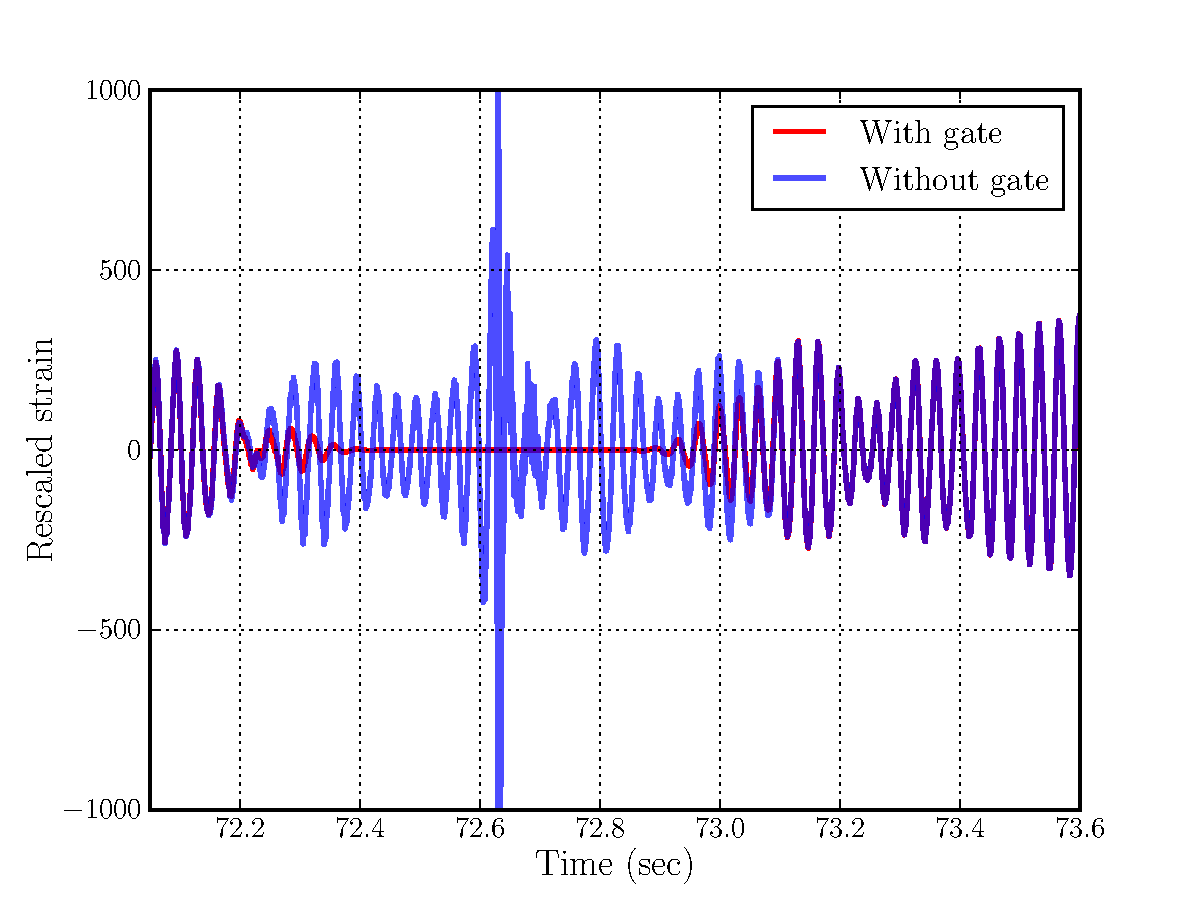
\includegraphics[width=0.9\linewidth]{images/2_searches/autogating.pdf}
    \caption{Gating a very loud noise transient. The detector strain has been rescaled by a factor of $10^{21}$ and the glitch has a peak magnitude over $5,000$. The blue line shows the data before applying the Tukey window and the red shows the data after applying the Tukey window. Note the smooth decrease in data amplitude at the edges of the windowing function. Image taken from~\cite{PyCBC:2016}.}
    \label{2:fig:autogating}
\end{figure}
%

Gating occurs automatically in \gwadj searches in a process called `auto-gating'. Auto-gating in PyCBC Live zeroes only $0.25$ seconds of data with a taper of $0.25$ seconds on either side. Auto-gating will completely remove the delta-function glitch and will prevent the ringing effect, removing the triggers caused by the glitch.

\subsection{\label{2:sec:coincidence-test}Coincidence tests}

Non-Gaussian transients in our detector data lead to greatly increased possibility for a \gwadj detector to report detections of \gwadj signals caused by non-astrophysical sources. If, after our signal-consistency tests, a glitch has a large SNR we are unable to make a distinction between it and a real event.

In terms of the optimal detection statistic, we must include further components which can reject glitches while ensuring we continue to detect all possible real events. The most powerful method for confirming the detection in one detector is the coincidental detection of the same signal in another detector. We call this a \textit{coincidence test}; the requirement that for a signal to be considered real, it must have been observed in multiple detectors.

In a two detector example, for example LIGO-Hanford and LIGO-Livingston, the signal seen by both detectors will not be exactly the same. The detectors are located approximately $3,000 \, \text{km}$ from one another, (Figure~\ref{2:fig:observatories}) and we know \gws propagate at the speed of light (Section~\ref{1:sec:keplerian_derivation}).
%
\begin{figure}
    \centering
    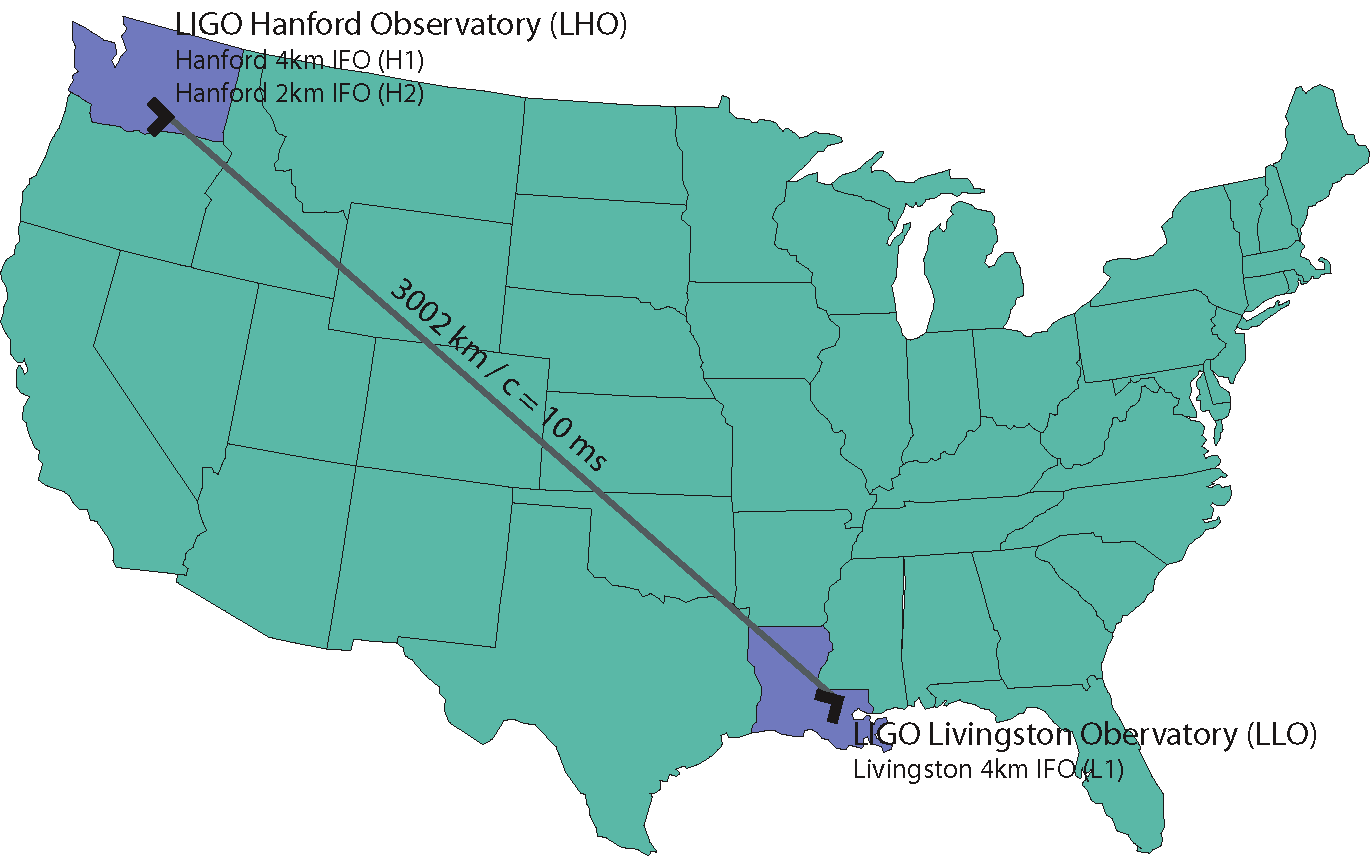
\includegraphics[width=0.8\linewidth]{images/2_searches/observatories.png}
    \caption{The two LIGO detectors locations and orientations, separated by approximately $3,000 \, \text{km}$. Taken from~\cite{Brown_Thesis:2004}.}
    \label{2:fig:observatories}
\end{figure}
%
Therefore, we can expect a maximum delay between single-detector detections of $10 \, \text{ms}$. For the coincidence test, we must allow a window between single detector triggers of this light travel time. An additional coincidence requirement in PyCBC is the intrinsic parameters of the two single detector triggers being the same, i.e. they have seen the same gravitational waveform.


\subsection{\label{2:sec:ranking-statistic}Ranking statistic}

Finally, we can combine all these components to create a ranking statistic to use as the detection statistic for identifying \gwadj signals from \gwadj detector data. The likelihood ratio is calculated using the signal and noise event rate densities, defined as~\cite{PyCBC_global:2020}
%
\begin{equation}
    r_{s}(\kappa) = \frac{\text{Number of signal events}}{\text{Volume} \times \text{Time}},
\end{equation}
%
\begin{equation}
    r_{n}(\kappa) = \frac{\text{Number of noise events}}{\text{Volume} \times \text{Time}}.
\end{equation}
%
We compare the number of signal and noise events over the total Volume-Time (VT) observed, the number of signal events should increase with an increase in both volume and time, but the number of noise events will not change with an increase in volume, only time. We use the volume in the noise event rate density calculation to allow us to simply compare the two rates as the VT cancels in likelihood ratio
%
\begin{equation}
    \Lambda(\vec{\kappa}) = \frac{r_{s}(\vec{\kappa})}{r_{n}(\vec{\kappa})},
\end{equation}
%
where $\vec{\kappa}$ is a set of parameters
%
\begin{equation}
    \vec{\kappa} = \left\{ \left[\rho_{d}, \chi^{2}_{d}, \chi^{2}_{d, sg}, \sigma_{d}\right], \vec{\theta}, \left[\mathfrak{A}_{d_{1}d_{2}}, \delta t_{d_{1}d_{2}}, \delta\phi_{d_{1}d_{2}}\right] \right\}.
\end{equation}
%
$\vec{\kappa}$ contains three categories of parameter: first, the single detector trigger parameters for each detector $d$, SNR, Allen-$\chi^{2}$, sine-Gaussian $\chi^{2}$ and template sensitivity ($\sigma_{d}$); next, the intrinsic template parameters $\vec{\theta}$ and; the coincident trigger parameters, amplitude ratio ($\mathfrak{A}_{ab}$), time of arrival difference ($\delta t_{ab}$) and phase difference ($\delta \phi_{ab}$) between two detectors $d_{1}$ and $d_{2}$.

Again, it is natural to use the log-likelihood ratio due to the order of magnitude difference between the event rate densities
%
\begin{equation}
    R(\vec{\kappa}) = \log \Lambda(\vec{\kappa}) = \log r_{s}(\vec{\kappa}) - \log r_{n}(\vec{\kappa}).
\end{equation}
%
We call the log-likelihood detection statistic the ranking statistic, which is constructed from a noise model and signal model. The PyCBC noise and signal models have changed over the course of the \gwadj search history. We will describe the models used in~\cite{PyCBC:2016}, the first iteration of the \texttt{PyCBC} search for \cbcs.

\subsubsection{\label{2:sec:pycbc-2016}PyCBC}

The \texttt{PyCBC} search pipeline ranked single detector triggers by their SNR and $\chi^{2}$ values to create a re-weighted SNR, $\hat{\rho}_{d}$, for each detector. The \texttt{PyCBC} search pipeline ranking statistic noise event rate model provides information on how likely an event is to be caused by noise. The noise event rate model used by the \texttt{PyCBC} search pipeline was a simple quadrature sum of single detector re-weighted SNRs,
%
\begin{equation}
    \hat{\rho}^{2} = \sqrt{\hat{\rho}^{2}_{d_{1}} + \hat{\rho}^{2}_{d_{2}}},
    \label{2:eq:PyCBC_noise_model}
\end{equation}
%
where a large $\hat{\rho}^{2}$ indicates a more significant event, less likely to be caused by noise.

The \texttt{PyCBC} search pipeline had no signal event rate model, and so the ranking statistic was simply the noise event rate model presented above. As detailed in~\cite{PyCBC:2016}, this ranking statistic was shown to `downrank' all triggers below a re-weighted SNR of $6$ in both a Gaussian noise simulation and the $6^{th}$ science run of LIGO~\cite{rw_snr_eq:2012}. We note that in this case there are $0$ real signals in the data and therefore this noise model has been applied to only noise triggers.

\subsection{\label{2:sec:background-estimation}Candidate event significance}

We can define some threshold at which a coincident trigger with ranking statistic value above this threshold can be preliminary considered to be a \gwadj event, we refer to these coincident triggers as \textit{candidates}. We define the \textit{significance} of the candidate as the \textit{false-alarm rate}. False alarms are coincident triggers that have been cause entirely by noise, with no astrophysical origin. The rate of false alarms depends on the search pipeline's response to detector noise and must be measured empirically.

The PyCBC search pipeline measures the false-alarm rate using `time slides'. As discussed in Section~\ref{2:sec:coincidence-test}, a coincident trigger can only be formed if the triggers are within the light travel time window. Therefore, if a coincidence is made between two single detector triggers outside this window it \textbf{must} be caused by detector noise and not an astrophysical signal. To measure the background rate of coincident triggers, we can take the triggers from the first detector and count all the coincidences made with the triggers from the second detector after shifting the time in the second detector by greater than the light travel time window. This ensures that any coincidences made cannot possibly have been due to a real signal because the coincidences will have occurred outside the light travel time window. An example of a background coincidence by these time slides for the three detector case can be seen in Figure~\ref{2:fig:timeslides}.
%
\begin{figure}
    \centering
    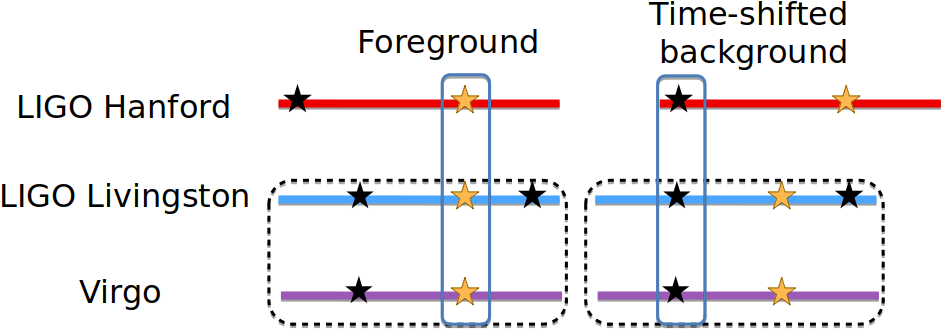
\includegraphics[width=0.9\linewidth]{images/2_searches/TimeslideExample.png}
    \caption{The time-sliding process carried out by the PyCBC search to generate a background distribution of candidate events. The foreground, real \gwadj event, is shown as a golden star and is the coincidence between three detectors with a single detector trigger in each which falls within the allowed light travel time of the detector network. The dashed black box indicates a time slide being made where two detectors have their data shifted by an interval greater than the allowed light travel time window to produce events which can only be caused by non-astrophysical noise sources. An example of a background event is shown as the three black stars in the blue box on the right image. Taken from~\cite{PyCBC_global:2020}.}
    \label{2:fig:timeslides}
\end{figure}
%

The time sliding procedure is repeated many times to produce a large sample of false-alarm coincidences, which are used to compute the false-alarm rate as a function of the ranking statistic.

To measure the significance of each candidate event, we assign a p-value. In our pipeline, the p-value of a candidate event is the probability that there are one or more false-alarm events that have a ranking statistic value greater than or equal to the ranking statistic of the detector value, $p_{b} = P(R_{FA} \ge R_{CE})$. The p-values of candidate events are calculated under the null hypothesis that \textit{all} triggers are seen due to noise. To confidently claim the candidate event as real, we must demonstrate that the null hypothesis given the candidate event ranking statistic value is highly improbable (the p-value is small).

We can do this by measuring the number of noise background events, $n_{b}$, that have a ranking statistic value higher than the candidate event. If we do this for all ranking statistic values we can build up a mapping of ranking statistic to false-alarm rate. The function $n_{b}(R)$ gives the number of background events with a ranking statistic value higher than $R$, the ranking statistic value. The probability that one or more background events are found above $R$ given the observing time $T$ and the background time $T_{b}$ is~\cite{PyCBC:2016}
%
\begin{equation}
    p(\ge 1 \, \text{above} R|T, T_{b})_{0} = 1 - \exp \left[\frac{-T(1 + n_{b}(R))}{T_{b}}\right].
\end{equation}
%
The background time will equal $T_{b} = T^{2}/\delta$ where $\delta$ is the time-slide interval. We can produce a very large amount of background data from a relatively small period of observing data, fifteen days of coincident data with a time-slide interval of $0.1$ seconds allows us to measure false-alarm rates of $1$ in $200,000$ years.

Finally, we can express the mapping of false-alarm rate to ranking statistic as
%
\begin{equation}
    \text{FAR}(R^{*}) = \int r_{n}(\vec{\kappa}) \Theta(R(\vec{\kappa}) - R^{*}) d^{n}\vec{\kappa},
    \label{2:eq:far_mapping}
\end{equation}
%
where $\Theta$ is the Heaviside step function
%
\begin{equation}
    \Theta(x) =
    \begin{cases} 
        0 & \text{if } x < 0 \\
        1 & \text{if } x \geq 0,
    \end{cases}
\end{equation}
%
and the false-alarm rate at the ranking statistic value $R^{*}$ is being calculated by integrating over all possible background events and summing up the events that have a ranking statistic greater than or equal to $R^{*}$, the ranking statistic threshold. The optimal ranking statistic will maximise the expected number of coincident events due to signals recovered above $R^{*}$.

\section{\label{2:sec:gw-pipelines}\Gwadj search pipelines}

We can develop the idea of a \gwadj search pipeline by describing the structure of the \texttt{PyCBC}~\cite{PyCBC:2016} search pipeline and how \gwadj events are identified from the initial \gwadj data using all the techniques described previously in this chapter.

\subsection{\label{2:sec:searching-for-gw-with-pycbc}\texttt{PyCBC}}
The flow chart describing the structure of the \texttt{PyCBC} pipeline has been taken from the \texttt{PyCBC} paper and can be seen in Figure~\ref{2:fig:pycbc-flowchart}. We follow this flowchart in our description of the search pipeline.
%
\begin{figure}
    \centering
    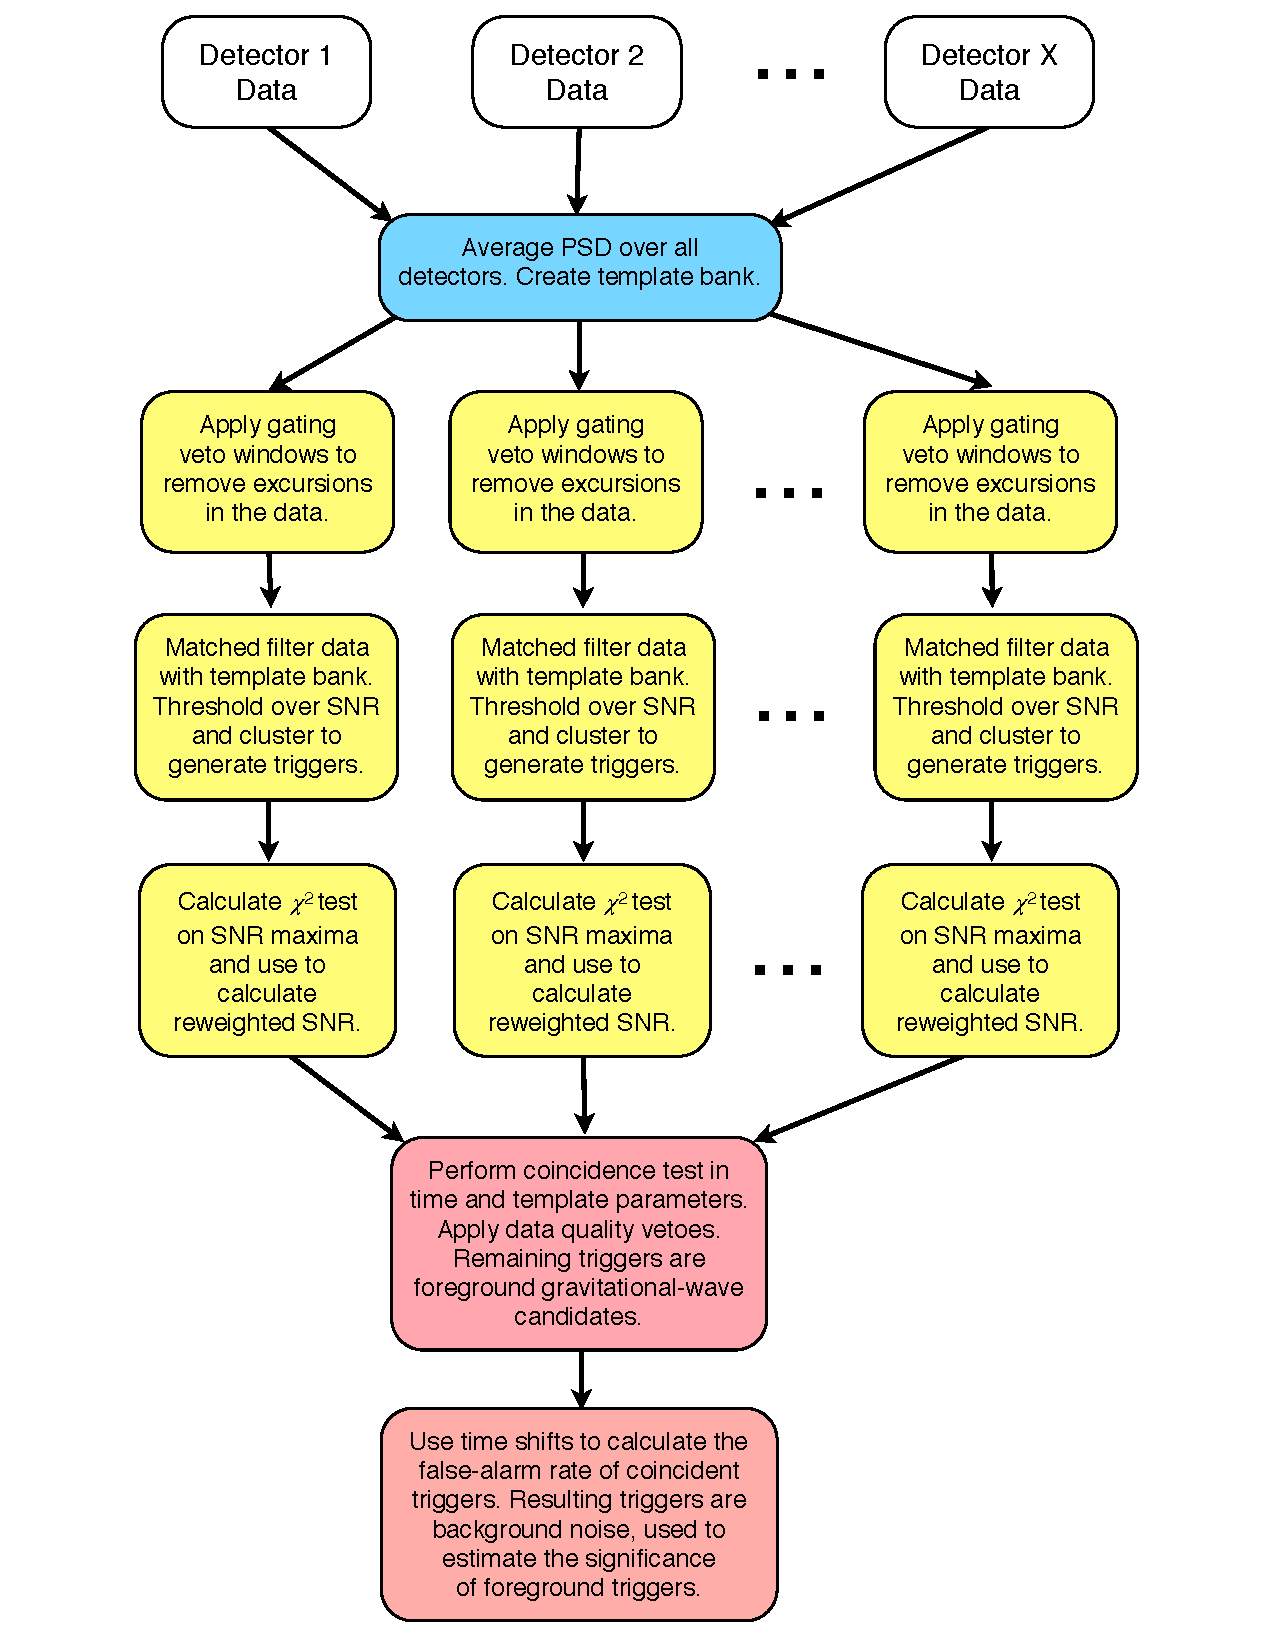
\includegraphics[width=1.0\linewidth]{images/2_searches/pycbc_flowchart.pdf}
    \caption{The structure of the \texttt{PyCBC} search pipeline for \gws. Taken from~\cite{PyCBC:2016}.}
    \label{2:fig:pycbc-flowchart}
\end{figure}







\subsubsection{Template bank generation}

A key consideration for \gwadj search pipelines is computational cost. A greater computational cost requires more time to analyse \gwadj data, alongside greater monetary cost and carbon emission cost. The dominant cost for modelled searches is matched filtering. Therefore, the number of templates in the template bank is proportional to the computational cost of the search. The number of templates is tuned to balance a minimal loss in matched filter SNR with the computational cost.

The template bank in the PyCBC search is shared between all detectors to allow a coincidence requirement of triggers sharing the same template between detectors. The template bank is generated given a power spectral density (PSD) and therefore we must create a PSD that is averaged over time for all detectors. The PSD is measured every $2048 \, \text{seconds}$ independently in each detector using Welch's method and taking the median average, this gives $N$ power spectra $S_{n}$ for each detector. The harmonic mean PSD for a single detector across all analysis time is then found
%
\begin{equation}
    S_{n}^{\text{harmonic}}(f_{k}) = N / \sum^{N}_{i = 1} \frac{1}{S^{i}_{n}(f_{k})},
\end{equation}
%
and using the same method we average across all detector harmonic mean PSDs to get an estimated PSD across all time and detectors to use for template bank generation. This PSD estimate only need to be re-generated when the detector's noise PSD has changed significantly, which will typically only happen when the detectors are physically changed or upgraded.

The \texttt{PyCBC} template bank is placed with a minimum match of $0.97$ between any signal and the template bank. The loss in sensitivity due to this minimum match limit is equal to the minimum-match cubed and is ${\simeq}10\%$. The template bank covers a four dimensional parameter space of two component masses and aligned spins. The PyCBC template bank was generated using a combined geometric-based aligned-spin algorithm~\cite{Harry_Lundgren:2012, Harry_precession:2013} and a stochastic algorithm~\cite{Ajith:2012, Privitera:2013}, described in~\cite{pycbc_template_bank:2016}.

A third observing run template bank can be seen plotted in the $m_{1}\text{--}m_{2}$ parameter space in Figure~\ref{2:fig:pycbc-o3-template-bank} which contains $428,725$ unique templates.
%
\begin{figure}
    \centering
    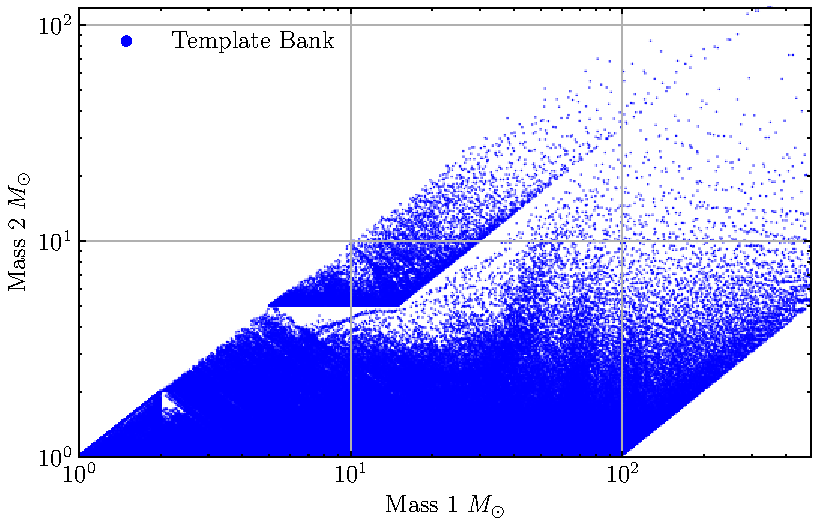
\includegraphics[width=0.75\linewidth]{images/2_searches/H1L1V1-PLOT_BANK.pdf}
    \caption{An example of a template bank used by the \texttt{PyCBC} search pipeline that has been generated from a single block of data and has been created in the four dimensional component mass and aligned spin parameter space. It consists of $428,725$ templates.}
    \label{2:fig:pycbc-o3-template-bank}
\end{figure}
%






\subsubsection{Matched filtering and clustering}

The matched filter between template bank and data is performed on each block of data to create a list of single detector triggers. Triggers are only stored if their matched filter SNR is greater than $5.5$. Suppose we have a trigger with an SNR of $10.0$, according to our template bank minimum match we should have at least one additional trigger (and indeed have many) above the SNR threshold for a nearby template. To prevent the recording of multiple triggers from different templates for the same candidate event, we use a \textit{time clustering} algorithm which selects and keeps only the highest SNR trigger in a predefined time window. Another clustering algorithm, is employed to trigger across the template bank to prevent the triggering of a loud glitch in one region of the template bank from subduing a real signal trigger in a completely different region.

\subsubsection{Signal consistency test}

The triggers then have the $\chi^{2}$ test~\cite{Allen_Chi:2005} applied to ensure consistency in the signal power distribution. The $\chi^{2}$ test values are calculated for each SNR trigger found by the template bank (Equation~\ref{2:eq:reduced_chisq}) and used to re-weight SNR values to obtain new SNR values for each trigger. An example of the SNR and $\chi^{2}$ time series from a loud signal can be seen in Figure~\ref{2:fig:snr-timeseries}.
%
\begin{figure}
    \centering
    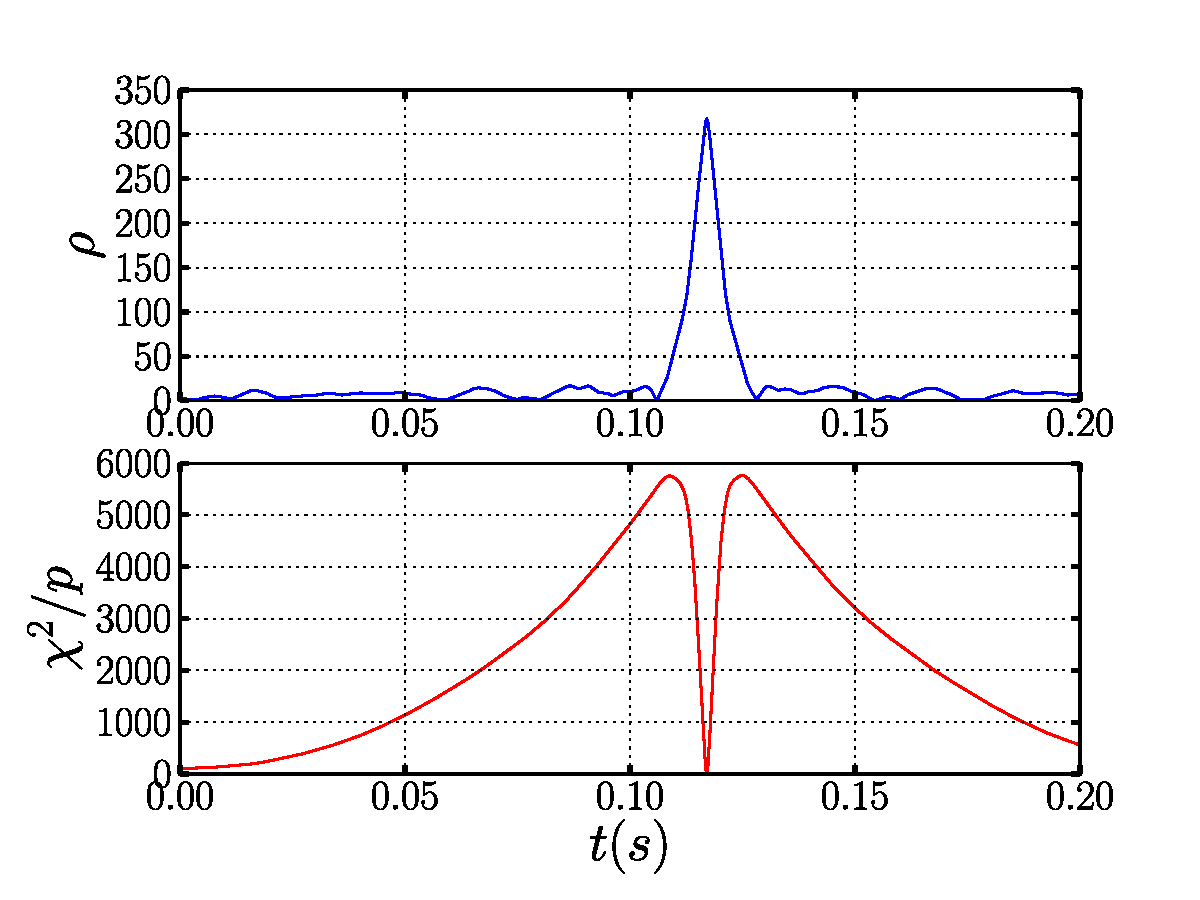
\includegraphics[width=0.75\linewidth]{images/2_searches/ihope_snr_timeseries.pdf}
    \caption{An SNR time series and $\chi^{2}$ time series for a simulated compact binary coalescence injected into S5~\cite{S5:2012} data with an SNR of $300$. Taken from~\cite{IHOPE:2012zx}.}
    \label{2:fig:snr-timeseries}
\end{figure}
%

\subsubsection{Coincidence tests}

Single detector triggers are combined and evaluated based on their trigger times and template parameters, triggers that have been found within the maximum light travel time between the two detectors ($10 \, \text{ms}$ for LIGO-Hanford and LIGO-Livingston) with an exactly matching template can be considered to originate from the same \gwadj signal~\cite{Robinson:2008}. The result of this process is a list of coincident triggers found with SNR above the threshold in two or more detectors, with exact template parameters across detectors.

\subsubsection{Generate background, rank triggers, establish significance and estimate search sensitivity}

The ranking statistic and false-alarm rates are calculated for each of these triggers as described in the previous section, using a quadrature sum of the reweighted SNR in each detector. The sensitivity of the search pipeline can be evaluated by injecting many simulated \gwadj signals into the data and recovering them with the search pipeline. The most realistic injections are hardware injections~\cite{Brown:2003, Biwer:2016} in which an actuator exerts a force on the end test mass to simulate the response of a real \gwadj signal. These injections are rarely performed because the data is now contaminated and cannot be used to search for real \gwadj signals. The injections used for large scale injection campaigns are software injections, in which the \gwadj signal is added to the data. These injections are added to add detectors with the correct time, phase, and amplitude differences and are placed so as to probe the full population of potential \gwadj events. The injection campaigns are a very powerful tool that can reveal search pipeline sensitivity, and we have used them extensively throughout this thesis to test the sensitivity increase of changes made to search pipelines.
